% !TEX root = tnnls_relation_gait.tex

\ifx\allfiles\undefined
    % !TEX root = tnnls_relation_gait.tex

%% bare_jrnl.tex
%% V1.4b
%% 2015/08/26
%% by Michael Shell
%% see http://www.michaelshell.org/
%% for current contact information.
%%
%% This is a skeleton file demonstrating the use of IEEEtran.cls
%% (requires IEEEtran.cls version 1.8b or later) with an IEEE
%% journal paper.
%%
%% Support sites:
%% http://www.michaelshell.org/tex/ieeetran/
%% http://www.ctan.org/pkg/ieeetran
%% and
%% http://www.ieee.org/

%%*************************************************************************
%% Legal Notice:
%% This code is offered as-is without any warranty either expressed or
%% implied; without even the implied warranty of MERCHANTABILITY or
%% FITNESS FOR A PARTICULAR PURPOSE!
%% User assumes all risk.
%% In no event shall the IEEE or any contributor to this code be liable for
%% any damages or losses, including, but not limited to, incidental,
%% consequential, or any other damages, resulting from the use or misuse
%% of any information contained here.
%%
%% All comments are the opinions of their respective authors and are not
%% necessarily endorsed by the IEEE.
%%
%% This work is distributed under the LaTeX Project Public License (LPPL)
%% ( http://www.latex-project.org/ ) version 1.3, and may be freely used,
%% distributed and modified. A copy of the LPPL, version 1.3, is included
%% in the base LaTeX documentation of all distributions of LaTeX released
%% 2003/12/01 or later.
%% Retain all contribution notices and credits.
%% ** Modified files should be clearly indicated as such, including  **
%% ** renaming them and changing author support contact information. **
%%*************************************************************************


% *** Authors should verify (and, if needed, correct) their LaTeX system  ***
% *** with the testflow diagnostic prior to trusting their LaTeX platform ***
% *** with production work. The IEEE's font choices and paper sizes can   ***
% *** trigger bugs that do not appear when using other class files.       ***                          ***
% The testflow support page is at:
% http://www.michaelshell.org/tex/testflow/

\documentclass[journal]{IEEEtran}
%
% If IEEEtran.cls has not been installed into the LaTeX system files,
% manually specify the path to it like:
% \documentclass[journal]{../sty/IEEEtran}

% Some very useful LaTeX packages include:
% (uncomment the ones you want to load)

% *** MISC UTILITY PACKAGES ***
%
%\usepackage{ifpdf}
% Heiko Oberdiek's ifpdf.sty is very useful if you need conditional
% compilation based on whether the output is pdf or dvi.
% usage:
% \ifpdf
%   % pdf code
% \else
%   % dvi code
% \fi
% The latest version of ifpdf.sty can be obtained from:
% http://www.ctan.org/pkg/ifpdf
% Also, note that IEEEtran.cls V1.7 and later provides a builtin
% \ifCLASSINFOpdf conditional that works the same way.
% When switching from latex to pdflatex and vice-versa, the compiler may
% have to be run twice to clear warning/error messages.

% *** CITATION PACKAGES ***

\usepackage{tabularx}
\usepackage{longtable}
\usepackage{threeparttable}
\usepackage{cite}

% cite.sty was written by Donald Arseneau
% V1.6 and later of IEEEtran pre-defines the format of the cite.sty package
% \cite{} output to follow that of the IEEE. Loading the cite package will
% result in citation numbers being automatically sorted and properly
% "compressed/ranged". e.g., [1], [9], [2], [7], [5], [6] without using
% cite.sty will become [1], [2], [5]--[7], [9] using cite.sty. cite.sty's
% \cite will automatically add leading space, if needed. Use cite.sty's
% noadjust option (cite.sty V3.8 and later) if you want to turn this off
% such as if a citation ever needs to be enclosed in parenthesis.
% cite.sty is already installed on most LaTeX systems. Be sure and use
% version 5.0 (2009-03-20) and later if using hyperref.sty.
% The latest version can be obtained at:
% http://www.ctan.org/pkg/cite
% The documentation is contained in the cite.sty file itself.

% *** GRAPHICS RELATED PACKAGES ***
%
\usepackage[pdftex]{graphicx}
\usepackage{rotating}
\ifCLASSINFOpdf
  % \usepackage[pdftex]{graphicx}
  % declare the path(s) where your graphic files are
  % \graphicspath{{../pdf/}{../jpeg/}}
  % and their extensions so you won't have to specify these with
  % every instance of \includegraphics
  % \DeclareGraphicsExtensions{.pdf,.jpeg,.png}
\else
  % or other class option (dvipsone, dvipdf, if not using dvips). graphicx
  % will default to the driver specified in the system graphics.cfg if no
  % driver is specified.
  % \usepackage[dvips]{graphicx}
  % declare the path(s) where your graphic files are
  % \graphicspath{{../eps/}}
  % and their extensions so you won't have to specify these with
  % every instance of \includegraphics
  % \DeclareGraphicsExtensions{.eps}
\fi
% graphicx was written by David Carlisle and Sebastian Rahtz. It is
% required if you want graphics, photos, etc. graphicx.sty is already
% installed on most LaTeX systems. The latest version and documentation
% can be obtained at:
% http://www.ctan.org/pkg/graphicx
% Another good source of documentation is "Using Imported Graphics in
% LaTeX2e" by Keith Reckdahl which can be found at:
% http://www.ctan.org/pkg/epslatex
%
% latex, and pdflatex in dvi mode, support graphics in encapsulated
% postscript (.eps) format. pdflatex in pdf mode supports graphics
% in .pdf, .jpeg, .png and .mps (metapost) formats. Users should ensure
% that all non-photo figures use a vector format (.eps, .pdf, .mps) and
% not a bitmapped formats (.jpeg, .png). The IEEE frowns on bitmapped formats
% which can result in "jaggedy"/blurry rendering of lines and letters as
% well as large increases in file sizes.
%
% You can find documentation about the pdfTeX application at:
% http://www.tug.org/applications/pdftex

% *** MATH PACKAGES ***
%
\usepackage{amsmath}
% A popular package from the American Mathematical Society that provides
% many useful and powerful commands for dealing with mathematics.
%
% Note that the amsmath package sets \interdisplaylinepenalty to 10000
% thus preventing page breaks from occurring within multiline equations. Use:
%\interdisplaylinepenalty=2500
% after loading amsmath to restore such page breaks as IEEEtran.cls normally
% does. amsmath.sty is already installed on most LaTeX systems. The latest
% version and documentation can be obtained at:
% http://www.ctan.org/pkg/amsmath

% *** SPECIALIZED LIST PACKAGES ***
%
\usepackage{algorithmic}
% algorithmic.sty was written by Peter Williams and Rogerio Brito.
% This package provides an algorithmic environment fo describing algorithms.
% You can use the algorithmic environment in-text or within a figure
% environment to provide for a floating algorithm. Do NOT use the algorithm
% floating environment provided by algorithm.sty (by the same authors) or
% algorithm2e.sty (by Christophe Fiorio) as the IEEE does not use dedicated
% algorithm float types and packages that provide these will not provide
% correct IEEE style captions. The latest version and documentation of
% algorithmic.sty can be obtained at:
% http://www.ctan.org/pkg/algorithms
% Also of interest may be the (relatively newer and more customizable)
% algorithmicx.sty package by Szasz Janos:
% http://www.ctan.org/pkg/algorithmicx

% *** ALIGNMENT PACKAGES ***
%
\usepackage{array}
% Frank Mittelbach's and David Carlisle's array.sty patches and improves
% the standard LaTeX2e array and tabular environments to provide better
% appearance and additional user controls. As the default LaTeX2e table
% generation code is lacking to the point of almost being broken with
% respect to the quality of the end results, all users are strongly
% advised to use an enhanced (at the very least that provided by array.sty)
% set of table tools. array.sty is already installed on most systems. The
% latest version and documentation can be obtained at:
% http://www.ctan.org/pkg/array

% IEEEtran contains the IEEEeqnarray family of commands that can be used to
% generate multiline equations as well as matrices, tables, etc., of high
% quality.

% *** SUBFIGURE PACKAGES ***
\usepackage[caption=false,font=footnotesize]{subfig}
%\ifCLASSOPTIONcompsoc
%  \usepackage[caption=false,font=normalsize,labelfont=sf,textfont=sf]{subfig}
%\else
%  \usepackage[caption=false,font=footnotesize]{subfig}
%\fi
% subfig.sty, written by Steven Douglas Cochran, is the modern replacement
% for subfigure.sty, the latter of which is no longer maintained and is
% incompatible with some LaTeX packages including fixltx2e. However,
% subfig.sty requires and automatically loads Axel Sommerfeldt's caption.sty
% which will override IEEEtran.cls' handling of captions and this will result
% in non-IEEE style figure/table captions. To prevent this problem, be sure
% and invoke subfig.sty's "caption=false" package option (available since
% subfig.sty version 1.3, 2005/06/28) as this is will preserve IEEEtran.cls
% handling of captions.
% Note that the Computer Society format requires a larger sans serif font
% than the serif footnote size font used in traditional IEEE formatting
% and thus the need to invoke different subfig.sty package options depending
% on whether compsoc mode has been enabled.
%
% The latest version and documentation of subfig.sty can be obtained at:
% http://www.ctan.org/pkg/subfig

% *** FLOAT PACKAGES ***
%
%\usepackage{fixltx2e}
% fixltx2e, the successor to the earlier fix2col.sty, was written by
% Frank Mittelbach and David Carlisle. This package corrects a few problems
% in the LaTeX2e kernel, the most notable of which is that in current
% LaTeX2e releases, the ordering of single and double column floats is not
% guaranteed to be preserved. Thus, an unpatched LaTeX2e can allow a
% single column figure to be placed prior to an earlier double column
% figure.
% Be aware that LaTeX2e kernels dated 2015 and later have fixltx2e.sty's
% corrections already built into the system in which case a warning will
% be issued if an attempt is made to load fixltx2e.sty as it is no longer
% needed.
% The latest version and documentation can be found at:
% http://www.ctan.org/pkg/fixltx2e

%\usepackage{stfloats}
% stfloats.sty was written by Sigitas Tolusis. This package gives LaTeX2e
% the ability to do double column floats at the bottom of the page as well
% as the top. (e.g., "\begin{figure*}[!b]" is not normally possible in
% LaTeX2e). It also provides a command:
%\fnbelowfloat
% to enable the placement of footnotes below bottom floats (the standard
% LaTeX2e kernel puts them above bottom floats). This is an invasive package
% which rewrites many portions of the LaTeX2e float routines. It may not work
% with other packages that modify the LaTeX2e float routines. The latest
% version and documentation can be obtained at:
% http://www.ctan.org/pkg/stfloats
% Do not use the stfloats baselinefloat ability as the IEEE does not allow
% \baselineskip to stretch. Authors submitting work to the IEEE should note
% that the IEEE rarely uses double column equations and that authors should try
% to avoid such use. Do not be tempted to use the cuted.sty or midfloat.sty
% packages (also by Sigitas Tolusis) as the IEEE does not format its papers in
% such ways.
% Do not attempt to use stfloats with fixltx2e as they are incompatible.
% Instead, use Morten Hogholm'a dblfloatfix which combines the features
% of both fixltx2e and stfloats:
%
% \usepackage{dblfloatfix}
% The latest version can be found at:
% http://www.ctan.org/pkg/dblfloatfix

%\ifCLASSOPTIONcaptionsoff
%  \usepackage[nomarkers]{endfloat}
% \let\MYoriglatexcaption\caption
% \renewcommand{\caption}[2][\relax]{\MYoriglatexcaption[#2]{#2}}
%\fi
% endfloat.sty was written by James Darrell McCauley, Jeff Goldberg and
% Axel Sommerfeldt. This package may be useful when used in conjunction with
% IEEEtran.cls'  captionsoff option. Some IEEE journals/societies require that
% submissions have lists of figures/tables at the end of the paper and that
% figures/tables without any captions are placed on a page by themselves at
% the end of the document. If needed, the draftcls IEEEtran class option or
% \CLASSINPUTbaselinestretch interface can be used to increase the line
% spacing as well. Be sure and use the nomarkers option of endfloat to
% prevent endfloat from "marking" where the figures would have been placed
% in the text. The two hack lines of code above are a slight modification of
% that suggested by in the endfloat docs (section 8.4.1) to ensure that
% the full captions always appear in the list of figures/tables - even if
% the user used the short optional argument of \caption[]{}.
% IEEE papers do not typically make use of \caption[]'s optional argument,
% so this should not be an issue. A similar trick can be used to disable
% captions of packages such as subfig.sty that lack options to turn off
% the subcaptions:
% For subfig.sty:
% \let\MYorigsubfloat\subfloat
% \renewcommand{\subfloat}[2][\relax]{\MYorigsubfloat[]{#2}}
% However, the above trick will not work if both optional arguments of
% the \subfloat command are used. Furthermore, there needs to be a
% description of each subfigure *somewhere* and endfloat does not add
% subfigure captions to its list of figures. Thus, the best approach is to
% avoid the use of subfigure captions (many IEEE journals avoid them anyway)
% and instead reference/explain all the subfigures within the main caption.
% The latest version of endfloat.sty and its documentation can obtained at:
% http://www.ctan.org/pkg/endfloat
%
% The IEEEtran \ifCLASSOPTIONcaptionsoff conditional can also be used
% later in the document, say, to conditionally put the References on a
% page by themselves.

% *** PDF, URL AND HYPERLINK PACKAGES ***
%
\usepackage{url}
% url.sty was written by Donald Arseneau. It provides better support for
% handling and breaking URLs. url.sty is already installed on most LaTeX
% systems. The latest version and documentation can be obtained at:
% http://www.ctan.org/pkg/url
% Basically, \url{my_url_here}.

% *** Do not adjust lengths that control margins, column widths, etc. ***
% *** Do not use packages that alter fonts (such as pslatex).         ***
% There should be no need to do such things with IEEEtran.cls V1.6 and later.
% (Unless specifically asked to do so by the journal or conference you plan
% to submit to, of course. )

% correct bad hyphenation here
% \hyphenation{op-tical net-works semi-conduc-tor}
\usepackage{enumerate}
\usepackage{multirow}
\usepackage{color}
\usepackage{threeparttable}
\usepackage{booktabs}
\newcommand{\minus}{\scalebox{0.75}[1.0]{$-$}}
\newcommand{\bftab}[1]{{\fontseries{b}\selectfont#1}}
\newcommand{\tabincell}[2]{\begin{tabular}{@{}#1@{}}#2\end{tabular}}
\newcommand{\etal}{\textit{et al}.}
\newcommand{\ie}{\textit{i.e.}}
\newcommand{\eg}{\textit{e.g.}}
\newcommand{\wrt}{\textit{w.r.t.}}
\newcommand{\vs}{\textit{vs.}}


\begin{document}
%
% paper title
% Titles are generally capitalized except for words such as a, an, and, as,
% at, but, by, for, in, nor, of, on, or, the, to and up, which are usually
% not capitalized unless they are the first or last word of the title.
% Linebreaks \\ can be used within to get better formatting as desired.
% Do not put math or special symbols in the title.
%\title{The Application and Research of Multi-modal Data in Auxiliary Diagnosis of Depression: A Survey
%}
\title{ Auxiliary Diagnosis of Depression Based on Multi-modal Data: A Survey
}
%%
%%
%% author names and IEEE memberships
%% note positions of commas and nonbreaking spaces ( ~ ) LaTeX will not break
%% a structure at a ~ so this keeps an author's name from being broken across
%% two lines.
%% use \thanks{} to gain access to the first footnote area
%% a separate \thanks must be used for each paragraph as LaTeX2e's \thanks
%% was not built to handle multiple paragraphs
%%
%
%\author{Saihui~Hou,
%	Xu~Liu,
%	Chunshui~Cao,
%	and~Yongzhen~Huang$^*$% <-this % stops a space
%	\thanks{$^*$ indicates the corresponding author.}% <-this % stops a space
%    \thanks{Saihui Hou and Yongzhen Huang is with School of Artificial Intelligence, Beijing Normal University, Beijing 100875, China. (Email: housaihui@bnu.edu.cn, huangyongzhen@bnu.edu.cn)}
%	\thanks{Xu Liu and Chunshui Cao are with Watrix Technology Limited Co. Ltd, Beijing 100088, China. (Email: xu.liu@watrix.ai, chunshuicao@watrix.ai)}
%    \thanks{This work is partially supported by the Fundamental Research Funds for the Central Universities.}
%    % \thanks{E-mail: housaihui@bnu.edu.cn, xu.liu@watrix.ai, chunshuicao@watrix.ai, huangyongzhen@bnu.edu.cn}
%	% \thanks{Manuscript received April 19, 2005; revised August 26, 2015.}
%}
%
%% note the % following the last \IEEEmembership and also \thanks -
%% these prevent an unwanted space from occurring between the last author name
%% and the end of the author line. i.e., if you had this:
%%
%% \author{....lastname \thanks{...} \thanks{...} }
%%                     ^------------^------------^----Do not want these spaces!
%%
%% a space would be appended to the last name and could cause every name on that
%% line to be shifted left slightly. This is one of those "LaTeX things". For
%% instance, "\textbf{A} \textbf{B}" will typeset as "A B" not "AB". To get
%% "AB" then you have to do: "\textbf{A}\textbf{B}"
%% \thanks is no different in this regard, so shield the last } of each \thanks
%% that ends a line with a % and do not let a space in before the next \thanks.
%% Spaces after \IEEEmembership other than the last one are OK (and needed) as
%% you are supposed to have spaces between the names. For what it is worth,
%% this is a minor point as most people would not even notice if the said evil
%% space somehow managed to creep in.
%
%% The paper headers
%\markboth{IEEE Transactions on Neural Networks and Learning Systems}%
%{Saihui Hou \MakeLowercase{\textit{et al.}}: GQAN: Towards the Interpretability of Silhouette-based Gait Recognition}
%% The only time the second header will appear is for the odd numbered pages
%% after the title page when using the twoside option.
%%
%% *** Note that you probably will NOT want to include the author's ***
%% *** name in the headers of peer review papers.                   ***
%% You can use \ifCLASSOPTIONpeerreview for conditional compilation here if
%% you desire.
%
%% If you want to put a publisher's ID mark on the page you can do it like
%% this:
%%\IEEEpubid{0000--0000/00\$00.00~\copyright~2015 IEEE}
%% Remember, if you use this you must call \IEEEpubidadjcol in the second
%% column for its text to clear the IEEEpubid mark.
%
%% use for special paper notices
%%\IEEEspecialpapernotice{(Invited Paper)}
%
%% make the title area
\maketitle

\fi

\section{Introduction}
%%%%%%%%%%%%%%%%%%%%%%%%%%%%%%%%%%%%%%%%%%%%%%%%%%%%%%%
%%%%%%%%%%%%%%%%%%%%%%%%%%%%%%%��ͮ������֪ʶǨ�ƣ�%%%%%%%%%%%%%%%%%%%%%%%%%%%%%%%%%%%%%%%%%%%%%%%%%
%Depression were the most common mental disorders, which brought great challenge to personal wellbeing and social economy around the world. According to World Health Organization (WHO), people with mental illness are among the main victims of the Covid-19 pandemic, with worldwide cases of depression rising by more than 25\% during the pandemic. Depression is a mental illness that does not directly lead to death, but many depressed people are unable to overcome their psychological barriers and choose to commit suicide. According to statistical surveys, the probability of suicide in depression is around 10-15\%. Given the high prevalence of depression and the risk of suicide, it is becoming increasingly important to find new diagnostic and treatment protocols.
%%%%%%%%%%%%%%%%%%%%%%%%%%%%%%%%%%%%%%%%%%%%%%%%%%%%%%%%%%%%%%%%%%%%%%%%%%%%%%%%%


Depression is one of the most common mental disorders~\cite{world2017depression,bhugra2004globalisation,rao2008understanding}, affecting more than 300 million people worldwide\cite{wang2021social}.
Depression is characterized by persistent grief, losing interest in things that are usually enjoyed, and the inability to participate in daily activities\cite{peveler2002depression}.
It will also make patients feel poorly and lose their living ability\cite{singh2009loneliness}.
Worse still, patients with severe symptoms have thoughts of self-harm or suicide~\cite{eisenberg2007prevalence,bergfeld2018treatment,hemming2019alexithymia}.
It is estimated that close to 70\% of depressed patients have had suicidal thoughts, and over 50\% have self-harmed\cite{huang2019prevalence}.
In short, the dangers of depression are staggering.

To alleviate the damage caused by depression, a timely and effective diagnosis is essential. However, there are three main challenges in the clinical diagnosis of depression:
(1) Lack of valid and accurate objective indicators. Compared with other physiological diseases, there are no objective and specific biochemical examination indexes, physiological data or medical images to diagnose and quantify depression. And clinicians can only make judgments based on the diagnostic criteria and their own working experience, as well as the clinical manifestations of patients~\cite{faust1988expert}, which may lead to biased diagnostic results due to some patients' uncooperative treatment and deliberate concealment of their true state.
(2) Serious shortage of medical resources. At present, there is a serious shortage of medical professionals and medical resources for the diagnosis and treatment of depression. In particular, in low- and middle-income countries, up to 75\% of patients do not receive timely diagnosis and treatment. In addition, face-to-face psychiatric consultations are time-consuming and inefficient, further exacerbating the shortage of resources for psychiatric treatment~\cite{cheng2022addressing,butryn2017shortage}.
(3) Deficiencies in social awareness. The low level of awareness of depression and the unconscious resistance or avoidance of mental illnesses can cause early depression to be underestimated or neglected, thus missing the best time for treatment, and may lead to the aggravation of the disease and increase the difficulty and complexity of treatment\cite{finch2000perceived,lauber2005recommendations,angermeyer2011biogenetic,pescosolido2013backbone}.

%To alleviate the damage caused by depression, timely and effective diagnosis is essential.
%However, there are four main challenges in the clinical diagnosis of depression:
%(1) Lack of valid and accurate objective indicators. In contrast to other physiological disorders, there are no objective and specific biochemical indicators, physiological signal data, or medical imaging to diagnose and quantify depression. Clinicians can only diagnose depression by interviewing patients, and at the same time, some patients do not cooperate with the diagnosis and deliberately conceal their true state, resulting in biased or misdiagnosed findings.
%
%
%
%However, there are various issues that need to be addressed in the clinical diagnosis of depression.
%On the one hand, compared to other physical diseases, there are no objective and specific biochemical indicators, physiological signal data, or medical imaging for diagnosing and quantifying depression.
%The clinician can only make a diagnosis by interviewing the patient and using assessment scales~\cite{faust1988expert}, which depend on the patient's level of cooperation.
%Nonetheless, social discrimination may make depressed people feel stressed\cite{finch2000perceived,lauber2005recommendations,angermeyer2011biogenetic,pescosolido2013backbone}.
%When face-to-face communication with a doctor or filling in the questionnaire, they may deliberately conceal some facts and that will lead to misdiagnosis.
%On the other hand, there is a severe shortage of professional psychiatrists required for the traditional diagnosis of depression worldwide\cite{cheng2022addressing,butryn2017shortage}, which prevents many patients from being diagnosed and treated promptly.


\begin{figure}
\centering
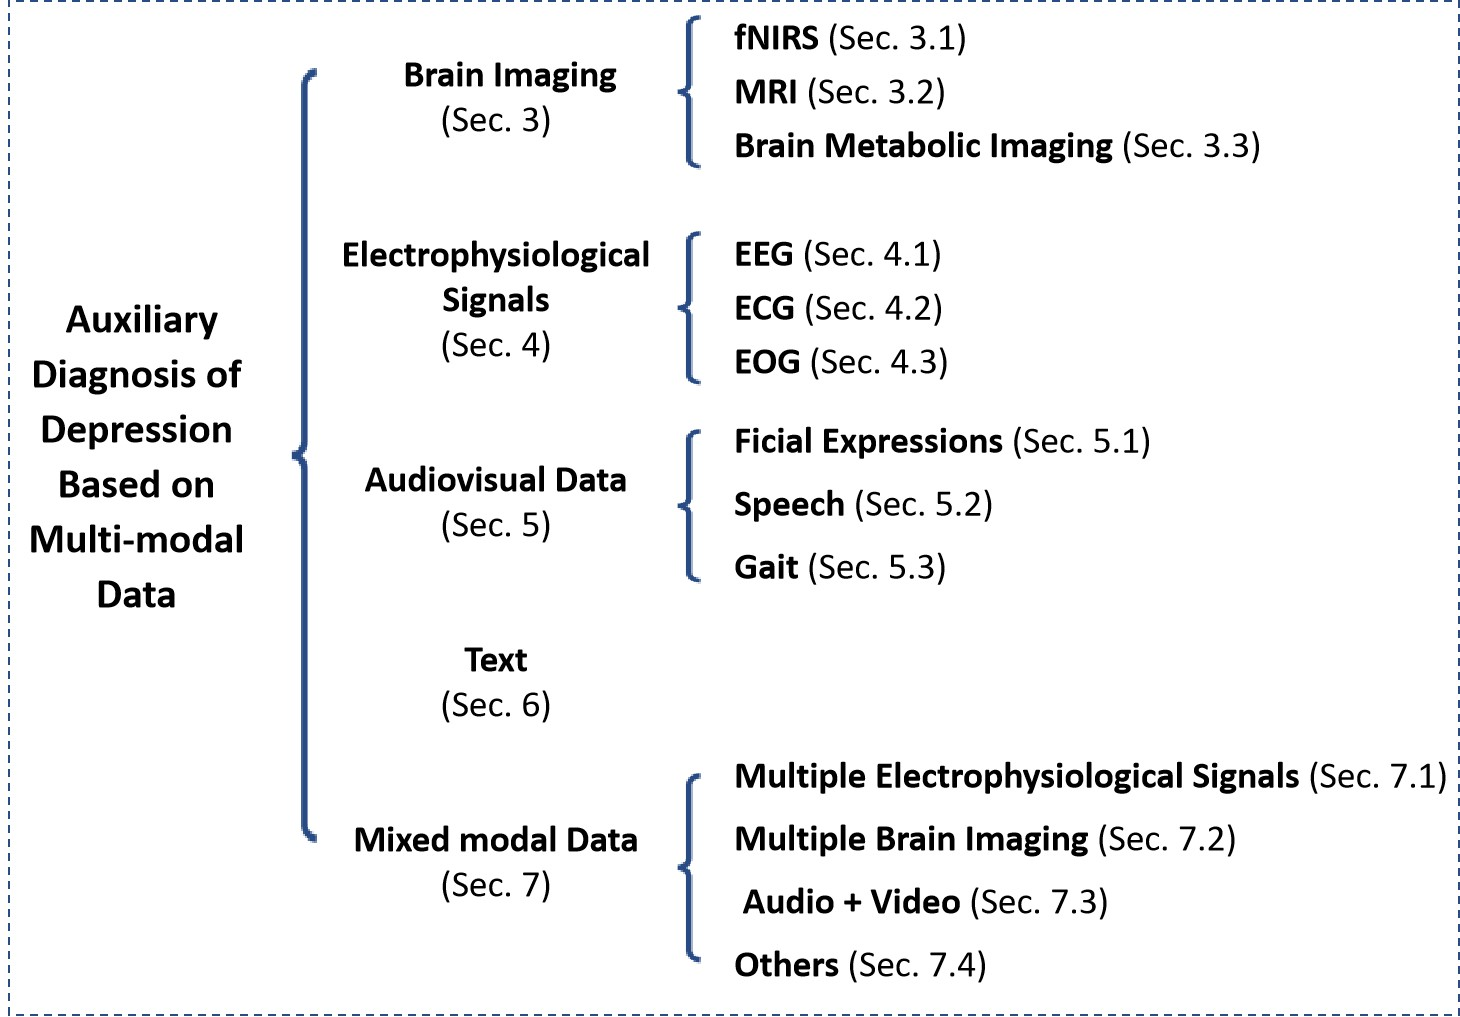
\includegraphics[width=1\linewidth]{Taxonomy.jpg}
\caption{The taxonomy of ancillary diagnosis of depression from the perspective of various categories of data.}
\label{Taxonomy}
\end{figure}
%recent ancillary diagnosis of depression (ADD) studies about the application of machine learning on various categories of data
%The taxonomy of occluded person Re-ID methods from the perspective of issues and solutions.



%The subjective factors of doctors or patients may cause misjudgements, which have an impact on the assessment of depression risk, and the search for objective methods has become the focus of research.
%In response to this circumstance, researchers have carried out studies on the evaluation of depression risk from several angles.
%By comparing the differences in physiological indicators and communication feedback exhibited between depressed and healthy people, they propose a series of machine learning-based methods to assist in depression identification.
%These methods focus on \emph{brain imaging}\cite{schnyer2017evaluating,sato2015machine,ramasubbu2016accuracy,vai2020predicting,wei2021functional},  \emph{electrophysiological signals}\cite{nilsonne2021eeg,shim2019machine,jiang2016predictability,li2016classification,kim2018automatic}, \emph{Audiovisual data}\cite{ma2016depaudionet,zhou2018visually,miao2021automatic},
%\emph{text}\cite{trotzek2018utilizing,park2015manifestation,yang2020big}, and \emph{multi-modal data}\cite{yang2017hybrid}.


%To address the difficulty of clinical diagnosis of depression, in recent years, researchers have proposed massive machine learning approaches based on the premise of comparing physiological indicators differences between depressed and healthy ones~\cite{luo2016big}.
%It not only avoids misdiagnosis or underdiagnosis due to patient non-cooperation to a large extent but also dramatically improves the efficiency of clinical diagnosis, reduces healthcare costs, and alleviates the shortage of healthcare resources.


To address the difficulty of clinical diagnosis of depression, in recent years, researchers have proposed massive machine learning approaches. With the help of machine learning, researchers extract effective features from depression patient data automatically, and then tap the intrinsic connection between depression clinical symptoms and patients' physiological signals, which has become an important direction for auxiliary diagnosis of  depression (ADD) ~\cite{luo2016big}. The following advantages exist for machine learning-based ADD:
(1) High efficiency: through the analysis of physiological signals of depression patients to establish objective diagnostic indicators, the efficiency of clinical diagnosis can be greatly improved by computer technology.
(2) Low interference: the machine learning method is used for automatically ADD, which eliminates the need for deliberate observation by clinicians and reduces the difficulty in depression diagnosis and treatment due to patient non-cooperation.
Despite the rapid evolution in this field, there is still no systematic study to review and discuss existing progress.
To fill this gap, a systematic analysis is carried out recent ancillary diagnosis of depression (ADD) studies about the application of machine learning on various categories of data, and the research process and methods of machine learning in ADD are summarized, and finally, the research directions and challenges in the future are presented.
As shown in Fig~\ref{Taxonomy}, we focus on the progress of the methods and potential research directions in five data contexts: \emph{brain imaging}\cite{schnyer2017evaluating,sato2015machine,ramasubbu2016accuracy,vai2020predicting,wei2021functional},  \emph{electrophysiological signals}\cite{nilsonne2021eeg,shim2019machine,jiang2016predictability,li2016classification,kim2018automatic}, \emph{Audiovisual data}\cite{ma2016depaudionet,zhou2018visually,miao2021automatic},
\emph{text}\cite{trotzek2018utilizing,park2015manifestation,yang2020big}, and \emph{mixed-modal data}\cite{yang2017hybrid}.
These commonly used representation forms of physiological signals are illustrated in Fig~\ref{common signals}
and some rough descriptions of them are as follows:


(1) \emph{Brain imaging:}
%%Brain function, brain structure, and brain metabolism imaging studies are the three main categories for brain imaging studies of depression.
%%%However, there are fewer structural and metabolic brain imaging investigations using depressed patients.
%%However, there are far more studies based on functional brain imaging than on the latter two.
%Brain imaging studies of depression are mainly divided into brain function, brain structure, and brain metabolism imaging studies. However, there are far more studies based on functional brain imaging of depressed patients,
%which mainly focus on dysfunction in the frontal lobe\cite{zhang2018multi,yamamura2016association,huang2017altered}, temporal lobe\cite{rolls2018effective}, amygdala\cite{zhu2018abnormal}, and cingulate gyrus\cite{gbyl2019cortical}.
%Functional magnetic resonance imaging (fMRI) is currently the main tool for studying functional brain imaging.
Brain imaging refers to the usually non-invasive or minimally invasive techniques that enable imaging the structure or function of the brain~\cite{lenartowicz2017brain}. This is achieved by scanning the subject��s brain with various precision instruments.
Its main data representations are: Functional Nearinfrared Spectroscopy (fNIRS), nuclebar Magnetic Resonance Imaging (MRI), etc. Studies have shown that, to some extent, brain imaging can identify different types of depression depending on the part of the brain affected~\cite{nestler2002neurobiology}.


(2) \emph{Electrophysiological signals:}
Electrophysiological signals are caused by changes in the membrane potential of individual cells~\cite{widmann2015digital}, which are usually recorded by metal electrodes placed on the body surface. The common electrophysiological signals that are of clinical interest are electroencephalography (EEG, tracing brain tissue activities), electrocardiography (ECG, recordings of the cardiac movement), and electrooculogram (EOG, examining the behavior of eyes). They have been used extensively to ADD because of their non-invasive detection and ease of use.
%Electrophysiological signals, which mainly include EEG,
%ECG, EOG, galvanic skin response, and body temperature,
%have been used extensively to diagnose depression because of
%their non-invasive detection and ease of use
% These signals arise from the membrane potential changes of electrically active cells, e.g., neurons in the brain controlling bodily functions, muscle cells enabling motion, pacemaker cells governing heart rhythm, and pancreatic cells responsible for insulin release. The common electrophysiological signals that are of clinical interest are electrocardiography (ECG, recordings of the cardiac movement), electroencephalography (EEG, tracing brain tissue activities), and electromyography (EMG, examining the behavior of muscle fibers or cells).

%Apart from using fMRI to assist in diagnosing depression, electrophysiological signals, especially electroencephalography(EEG), electrocardiography(ECG), electrodermal (EOG), and body temperature, have also received extensive attention\cite{trambaiolli2020resting}.
%EEG signals are most commonly used among them because of their great temporal resolution and sensitivity to minute changes in brain activity \cite{zeng2018eeg}.
%EEG-based methods for depression identification currently mostly use feature extraction with traditional classifier geometry, and some studies have also focused on convolutional neural networks.


%Electrophysiological signals to assist in the diagnosis of depression has also been heavily researched, mainly including electroencephalography, electrocardiography, electrodermal, gastric, ophthalmic, and body temperature. Among these, EEG signals are used most frequently due to their high temporal resolution and sensitivity to slight changes in brain activity [34]. EEG-based methods for depression identification currently mostly use feature extraction with traditional classifier geometry, and some studies have also focused on convolutional neural networks.


(3) \emph{Audiovisual data:}
Audiovisual data, whose forms mainly include facial expressions, speech, and gait, are captured by video and audio recording devices.
Audiovisual data based ADD is the first recognition method proposed by researchers and the most widely used method, which has the advantage of low acquisition cost but can achieve better recognition results.
%The audiovisual data based method was the first method proposed by researchers for ADD and is the most widely used method, with the advantage of low acquisition cost but better recognition results.


%Many researchers have used facial expression, speech, and gait to diagnose depression because depressed patients always exhibit abnormal behavior, such as sluggish facial expressions\cite{dai2012more}, frequent avoidance of eye contact, and speaking in short sentences with a flat tone\cite{kraepelin1921manic}. The model is more accurate based on the ease of obtaining data.

(4) \emph{Text:}
Text is the most direct vehicle for people to express their thoughts and emotions. Especially on social media platforms, people are more inclined to express their true feelings. Therefore, many researchers have examined the differences in textual expression between people with depression and normal ones in the context of social media platforms from a textual perspective~\cite{thomee2011mobile}.


(5) \emph{Mixed-modal data:}  In addition to the use of single physiological or behavioural data to assist in the diagnosis of depression, there have been many studies that have sought to employ multi-modal data for diagnosis  \cite{lalousis2021heterogeneity,meng2021bidirectional,toenders2022predicting}.
Multi-modal data have more features than unimodal data, which can give a more complete picture of the symptomatology of depressed patients.

\begin{figure}
\centering
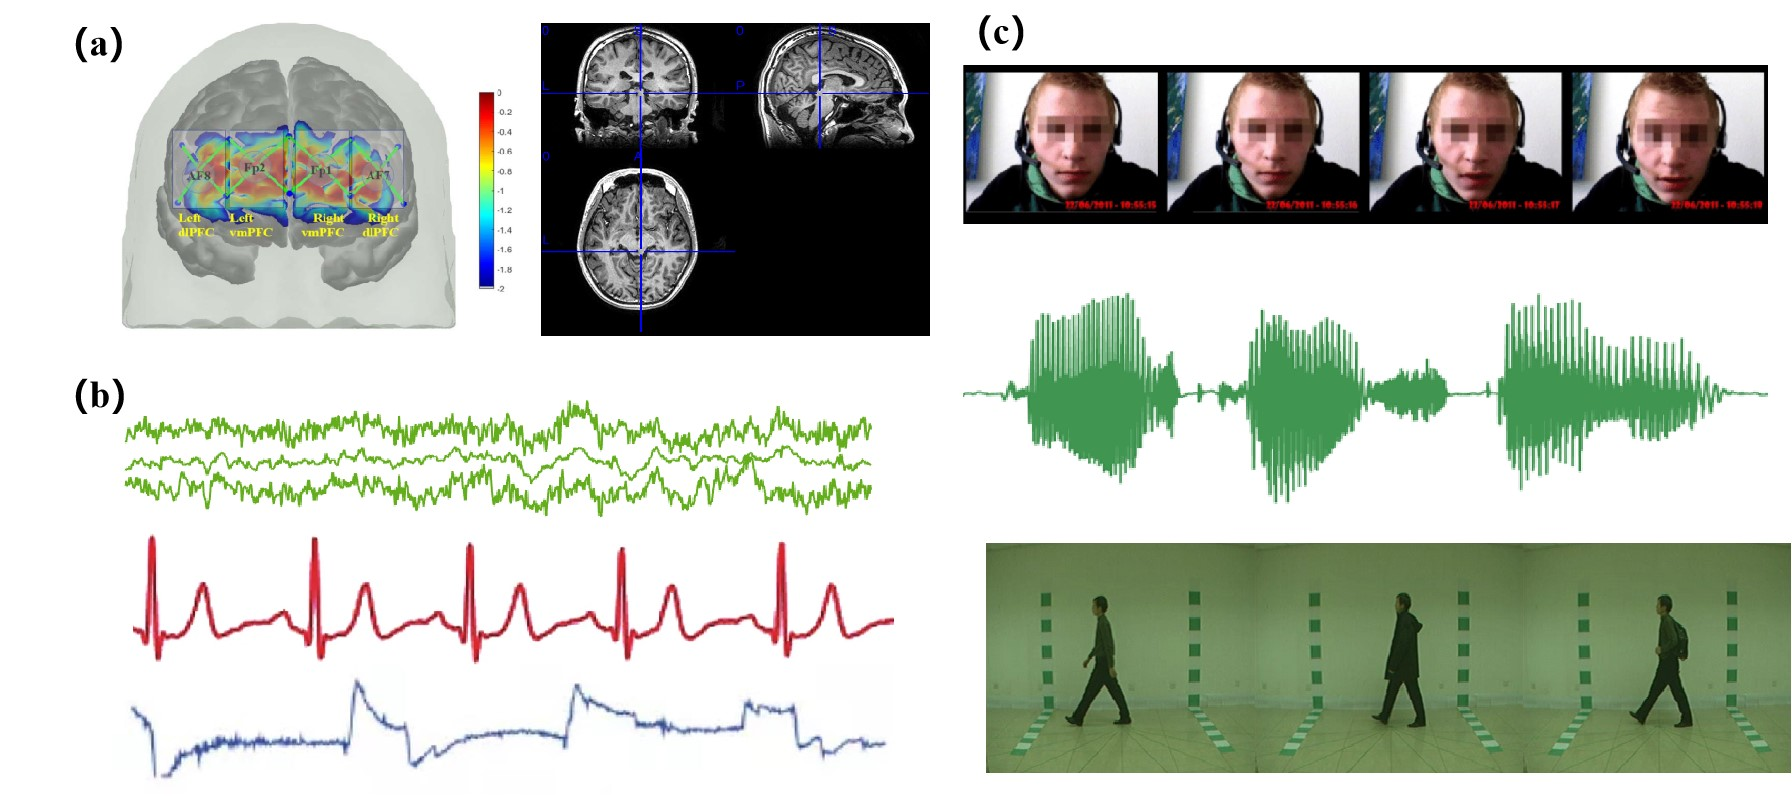
\includegraphics[width=1\linewidth]{raw_signals.jpg}
\caption{Common types of physiological signals: subgraphs $a-c$ represent brain imaging,electrophysiological signals, and audiovisual data, respectively. These categories in turn have different representations: fNIRS, MRI, EEG, ECG, EOG, facial expression, speech, and gait.}
\label{common signals}
\end{figure}


In this paper, we review the current state of research on machine learning in ADD regarding the five types mentioned above of data, with a focus on the progress of the use of machine learning techniques in different data contexts and potential research directions.
The main contributions of this study are threefold.

(1) To the best of our knowledge, this is the first comprehensive survey about ADD on different modalities of data, which will provide  researchers and clinical psychologists a better understanding of the use of machine learning for ADD.

(2) We provide an in-depth review of advanced ADD studies,
summarize and compare the performance of of different methods in each data modality.

(3) We summarize and analyze the advantages and disadvantages of different data types for ADD and give insights on promising research directions in this field.

The rest of this survey will be organized as follows:
Section 2 presents a summary of standard approaches to diagnosing clinical depression and abnormal changes in the physiology and behavior of depressed patients and introduces widely-used questionnaires, datasets, and metrics.
Section 3-7 provides an in-depth analysis of machine learning-based approaches to depression diagnosis from the perspective of different data types.
Section 8 provides insights into promising research directions. We conclude the survey in Section 9.


\ifx\allfiles\undefined
% !TEX root = tnnls_relation_gait.tex

% if have a single appendix:
%\appendix[Proof of the Zonklar Equations]
% or
%\appendix  % for no appendix heading
% do not use \section anymore after \appendix, only \section*
% is possibly needed

% use appendices with more than one appendix
% then use \section to start each appendix
% you must declare a \section before using any
% \subsection or using \label (\appendices by itself
% starts a section numbered zero.)
%

%\appendices
%\section{Proof of the First Zonklar Equation}
%Appendix one text goes here.
%
%% you can choose not to have a title for an appendix
%% if you want by leaving the argument blank
%\section{}
%Appendix two text goes here.

% use section* for acknowledgment
% \section*{Acknowledgment}
% The authors would like to thank Prof. Dongbin Zhao for his support to this work.

% Can use something like this to put references on a page
% by themselves when using endfloat and the captionsoff option.
\ifCLASSOPTIONcaptionsoff
  \newpage
\fi

% trigger a \newpage just before the given reference
% number - used to balance the columns on the last page
% adjust value as needed - may need to be readjusted if
% the document is modified later
%\IEEEtriggeratref{8}
% The "triggered" command can be changed if desired:
%\IEEEtriggercmd{\enlargethispage{-5in}}

% references section

% can use a bibliography generated by BibTeX as a .bbl file
% BibTeX documentation can be easily obtained at:
% http://mirror.ctan.org/biblio/bibtex/contrib/doc/
% The IEEEtran BibTeX style support page is at:
% http://www.michaelshell.org/tex/ieeetran/bibtex/
\bibliographystyle{IEEEtran}
% argument is your BibTeX string definitions and bibliography database(s)
\bibliography{IEEEabrv,tnnls_relation_gait}
%
% <OR> manually copy in the resultant .bbl file
% set second argument of \begin to the number of references
% (used to reserve space for the reference number labels box)
%\begin{thebibliography}{1}
%\bibitem{IEEEhowto:kopka}
%H.~Kopka and P.~W. Daly, \emph{A Guide to \LaTeX}, 3rd~ed.\hskip 1em plus
%  0.5em minus 0.4em\relax Harlow, England: Addison-Wesley, 1999.
%\end{thebibliography}

% biography section
%
% If you have an EPS/PDF photo (graphicx package needed) extra braces are
% needed around the contents of the optional argument to biography to prevent
% the LaTeX parser from getting confused when it sees the complicated
% \includegraphics command within an optional argument. (You could create
% your own custom macro containing the \includegraphics command to make things
% simpler here.)
%\begin{IEEEbiography}[{\includegraphics[width=1in,height=1.25in,clip,keepaspectratio]{mshell}}]{Michael Shell}
% or if you just want to reserve a space for a photo:

%\begin{IEEEbiography}{Michael Shell}
%Biography text here.
%\end{IEEEbiography}
%
%% if you will not have a photo at all:
%\begin{IEEEbiographynophoto}{John Doe}
%Biography text here.
%\end{IEEEbiographynophoto}

% insert where needed to balance the two columns on the last page with
% biographies
% \newpage

%\begin{IEEEbiographynophoto}{Jane Doe}
%Biography text here.
%\end{IEEEbiographynophoto}

%\begin{IEEEbiography}[{\includegraphics[width=1in,height=1.25in,clip,keepaspectratio]{photos/hsh.pdf}}]{Saihui Hou}
%% \begin{IEEEbiographynophoto}{Saihui Hou}
%	received the B.E. and Ph.D. degrees from University of Science and Technology of China in 2014 and 2019, respectively.
%    %
%    He is currently an Assistant Professor with School of Artificial Intelligence, Beijing Normal University.
%    %
%    His research interests include computer vision and machine learning.
%    %
%    He focuses on gait recognition which aims to identify different people according to the walking patterns.
%% \end{IEEEbiographynophoto}
%\end{IEEEbiography}
%
%\begin{IEEEbiography}[{\includegraphics[width=1in,height=1.25in,clip,keepaspectratio]{photos/lx.pdf}}]{Xu Liu}
%% \begin{IEEEbiographynophoto}{Xu Liu}
%	received the B.E. and Ph.D. degrees from University of Science and Technology of China in 2013 and 2018, respectively.
%    %
%    He is currently a Research Scientist with Watrix Technology Limited Co. Ltd.
%    %
%    His research interests include gait recognition, object detection and image segmentation.
%% \end{IEEEbiographynophoto}
%\end{IEEEbiography}
%
%\begin{IEEEbiography}[{\includegraphics[width=1in,height=1.25in,clip,keepaspectratio]{photos/ccs.pdf}}]{Chunshui Cao}
%% \begin{IEEEbiographynophoto}{Chunshui Cao}
%	received the B.E. and Ph.D. degrees from University of Science and Technology of China in 2013 and 2018, respectively.
%    %
%    During his Ph.D. study, he joined Center for Research on Intelligent Perception and Computing, National Laboratory of Pattern Recognition, Institute of Automation, Chinese Academy of Sciences.
%    %
%    From 2018 to 2020, he worked as a Postdoctoral Fellow with PBC School of Finance, Tsinghua University.
%    %
%    He is currently a Research Scientist with Watrix Technology Limited Co. Ltd.
%    %
%    His research interests include pattern recognition, computer vision and machine learning.
%% \end{IEEEbiographynophoto}
%\end{IEEEbiography}
%
%\begin{IEEEbiography}[{\includegraphics[width=1in,height=1.25in,clip,keepaspectratio]{photos/hyz.pdf}}]{Yongzhen Huang}
%% \begin{IEEEbiographynophoto}{Yongzhen Huang}
%	received the B.E. degree from Huazhong University of Science and Technology in 2006, and the Ph.D. degree from Institute of Automation, Chinese Academy of Sciences in 2011.
%    %
%    He is currently an Associate Professor with School of Artificial Intelligence, Beijing Normal University.
%    %
%    He has published one book and more than 80 papers at international journals and conferences such as TPAMI, IJCV, TIP, TSMCB, TMM, TCSVT, CVPR, ICCV, ECCV, NIPS, AAAI.
%    %
%    His research interests include pattern recognition, computer vision and machine learning.
%% \end{IEEEbiographynophoto}
%\end{IEEEbiography}


\end{document}

\fi
